\documentclass[11pt,letterpaper,notitlepage]{article}
\usepackage[left=1in,right=1in,top=1in,bottom=1in]{geometry}
\usepackage[dvipsnames]{xcolor}
\definecolor{darkblue}{RGB}{46,48,147}
\usepackage{hyperref}
\hypersetup{colorlinks=true,
            linkcolor=darkblue,
            urlcolor=darkblue,
            citecolor=darkblue}
\usepackage{xspace}
\usepackage{amsmath,amsfonts,amssymb}
\usepackage{lipsum}
\usepackage[utf8]{inputenc}
\usepackage[T1]{fontenc}
\usepackage{palatino}
\usepackage{mathpazo}
\usepackage{ifthen}
\newboolean{cms@italic}
\setboolean{cms@italic}{false}
\newboolean{cms@external}
\setboolean{cms@external}{false}
\usepackage[pazoGreek]{heppennames2}
\usepackage{ptdr-definitions}
\usepackage{lastpage}
\usepackage{fancyhdr}
\usepackage{graphicx}
\renewcommand{\headrulewidth}{0pt}
\lhead{Javier M. Duarte}
\rhead{Personal Statement}
\cfoot{\thepage}

\newcommand{\mycite}[1]{%
\ifthenelse{\equal{#1}{Khachatryan:2015pwa}}{\href{https://doi.org/10.1103/PhysRevD.91.052018}{\textbf{A.I.277}}}{}%
\ifthenelse{\equal{#1}{Anderson:2015tia}}{\href{https://doi.org/10.1016/j.nima.2014.11.041}{\textbf{A.I.311}}}{}%
\ifthenelse{\equal{#1}{Anderson:2015gha}}{\href{https://doi.org/10.1016/j.nima.2015.04.013}{\textbf{A.I.317}}}{}%
\ifthenelse{\equal{#1}{Anderson:2016ygg}}{\href{https://doi.org/10.1109/TNS.2016.2528166}{\textbf{A.I.373}}}{}%
\ifthenelse{\equal{#1}{Anderson:2016tiu}}{\href{https://doi.org/10.1016/j.nima.2015.11.129}{\textbf{A.I.396}}}{}%
\ifthenelse{\equal{#1}{Khachatryan:2016epu}}{\href{https://doi.org/10.1103/PhysRevD.95.012003}{\textbf{A.I.444}}}{}%
\ifthenelse{\equal{#1}{Sirunyan:2016iap}}{\href{https://doi.org/10.1016/j.physletb.2017.02.012}{\textbf{A.I.491} (293 citations)}}{}%
\ifthenelse{\equal{#1}{Sirunyan:2017nvi}}{\href{https://doi.org/10.1007/JHEP01(2018)097}{\textbf{A.I.567} (183 citations)}}{}%
\ifthenelse{\equal{#1}{Sirunyan:2017dgc}}{\href{https://doi.org/10.1103/PhysRevLett.120.071802}{\textbf{A.I.571} (154 citations)}}{}%
\ifthenelse{\equal{#1}{Sirunyan:2017eie}}{\href{https://doi.org/10.1016/j.physletb.2017.12.069}{\textbf{A.I.604}}}{}%
\ifthenelse{\equal{#1}{Duarte:2018ite}}{\href{https://doi.org/10.1088/1748-0221/13/07/P07027}{\textbf{A.I.644} (258 citations)}}{}%
\ifthenelse{\equal{#1}{Sirunyan:2018xlo}}{\href{https://doi.org/10.1007/JHEP08(2018)130}{\textbf{A.I.662} (250 citations)}}{}%
\ifthenelse{\equal{#1}{Sirunyan:2018kst}}{\href{https://doi.org/10.1103/PhysRevLett.121.121801}{\textbf{A.I.667} (622 citations)}}{}%
\ifthenelse{\equal{#1}{Sirunyan:2018ikr}}{\href{https://doi.org/10.1103/PhysRevD.99.012005}{\textbf{A.I.713} (26 citations)}}{}%
\ifthenelse{\equal{#1}{Sirunyan:2018koj}}{\href{https://doi.org/10.1140/epjc/s10052-019-6909-y}{\textbf{A.I.761}}}{}%
\ifthenelse{\equal{#1}{Sirunyan:2018sgc}}{\href{https://doi.org/10.1016/j.physletb.2019.03.059}{\textbf{A.I.762} (85 citations)}}{}%
\ifthenelse{\equal{#1}{Duarte:2019fta}}{\href{https://doi.org/10.1007/s41781-019-0027-2}{\textbf{A.I.794} (41 citations)}}{}%
\ifthenelse{\equal{#1}{Sirunyan:2019vxa}}{\href{https://doi.org/10.1103/PhysRevD.100.112007}{\textbf{A.I.817} (75 citations)}}{}%
\ifthenelse{\equal{#1}{Sirunyan:2019sgo}}{\href{https://doi.org/10.1103/PhysRevLett.123.231803}{\textbf{A.I.818} (44 citations)}}{}%
\ifthenelse{\equal{#1}{Moreno:2019bmu}}{\href{https://doi.org/10.1140/epjc/s10052-020-7608-4}{\textbf{A.I.824} (84 citations)}}{}%
\ifthenelse{\equal{#1}{Summers:2020xiy}}{\href{https://doi.org/10.1088/1748-0221/15/05/p05026}{\textbf{A.I.861} (41 citations)}}{}%
\ifthenelse{\equal{#1}{Sirunyan:2019vgj}}{\href{https://doi.org/10.1007/JHEP05(2020)033}{\textbf{A.I.866} (125 citations)}}{}%
\ifthenelse{\equal{#1}{Sirunyan:2019pnb}}{\href{https://doi.org/10.1016/j.physletb.2020.135448}{\textbf{A.I.875} (26 citations)}}{}%
\ifthenelse{\equal{#1}{Moreno:2019neq}}{\href{https://doi.org/10.1103/PhysRevD.102.012010}{\textbf{A.I.877} (49 citations)}}{}%
\ifthenelse{\equal{#1}{DiGuglielmo:2020eqx}}{\href{https://doi.org/10.1088/2632-2153/aba042}{\textbf{A.I.910} (44 citations)}}{}%
\ifthenelse{\equal{#1}{Sirunyan:2020hwz}}{\href{https://doi.org/10.1007/JHEP12(2020)085}{\textbf{A.I.911} (41 citations)}}{}%
\ifthenelse{\equal{#1}{Iiyama:2020wap}}{\href{https://doi.org/10.3389/fdata.2020.598927}{\textbf{A.I.915} (41 citations)}}{}%
\ifthenelse{\equal{#1}{Krupa:2020bwg}}{\href{https://doi.org/10.1088/2632-2153/abec21}{\textbf{A.I.930} (20 citations)}}{}%
\ifthenelse{\equal{#1}{Pata:2021oez}}{\href{https://doi.org/10.1140/epjc/s10052-021-09158-w}{\textbf{A.I.940} (48 citations)}}{}%
\ifthenelse{\equal{#1}{Aarrestad:2021zos}}{\href{https://doi.org/10.1088/2632-2153/ac0ea1}{\textbf{A.I.945} (39 citations)}}{}%
\ifthenelse{\equal{#1}{Hawks:2021ruw}}{\href{https://doi.org/10.3389/frai.2021.676564}{\textbf{A.I.949} (17 citations)}}{}%
\ifthenelse{\equal{#1}{DiGuglielmo:2021ide}}{\href{https://doi.org/10.1109/TNS.2021.3087100}{\textbf{A.I.952} (11 citations)}}{}%
\ifthenelse{\equal{#1}{John:2020sak}}{\href{https://doi.org/10.1103/PhysRevAccelBeams.24.104601}{\textbf{A.I.971} (13 citations)}}{}%
\ifthenelse{\equal{#1}{Dezoort:2021kfk}}{\href{https://doi.org/10.1007/s41781-021-00073-z}{\textbf{A.I.974} (21 citations)}}{}%
\ifthenelse{\equal{#1}{Zlokapa:2019tkn}}{\href{https://doi.org/10.1007/s42484-021-00054-w}{\textbf{A.I.975} (30 citations)}}{}%
\ifthenelse{\equal{#1}{CMS:2021juv}}{\href{https://doi.org/10.1103/PhysRevLett.127.261804}{\textbf{A.I.987} (11 citations)}}{}%
\ifthenelse{\equal{#1}{Kasieczka:2021xcg}}{\href{https://doi.org/10.1088/1361-6633/ac36b9}{\textbf{A.I.988} (70 citations)}}{}%
\ifthenelse{\equal{#1}{Aarrestad:2021oeb}}{\href{https://doi.org/10.21468/SciPostPhys.12.1.043}{\textbf{A.I.992} (35 citations)}}{}%
\ifthenelse{\equal{#1}{Chen:2021euv}}{\href{https://doi.org/10.1038/s41597-021-01109-0}{\textbf{A.I.993}}}{}%
\ifthenelse{\equal{#1}{Govorkova:2021utb}}{\href{https://doi.org/10.1038/s42256-022-00441-3}{\textbf{A.I.994}}}{}%
\ifthenelse{\equal{#1}{Jawahar:2021vyu}}{\href{https://doi.org/10.3389/fdata.2022.803685}{\textbf{A.I.996}}}{}%
\ifthenelse{\equal{#1}{Elabd:2021lgo}}{\href{https://doi.org/10.3389/fdata.2022.828666}{\textbf{A.I.1004}}}{}%
\ifthenelse{\equal{#1}{CMS:2021yhb}}{\href{https://doi.org/10.1007/JHEP03(2022)160}{\textbf{A.I.1006}}}{}%
\ifthenelse{\equal{#1}{CMS:2022nmn}}{\href{https://arxiv.org/abs/2205.06667}{\textbf{A.I.1028}}}{}%
\ifthenelse{\equal{#1}{CMS:2022dwd}}{\href{https://doi.org/10.1038/s41586-022-04892-x}{\textbf{A.I.1029}}}{}%
\ifthenelse{\equal{#1}{Touranakou:2022qrp}}{\href{https://doi.org/10.1088/2632-2153/ac7c56}{\textbf{A.I.1030}}}{}%
\ifthenelse{\equal{#1}{Deiana:2021niw}}{\href{https://doi.org/10.3389/fdata.2022.787421}{\textbf{A.II.1}}}{}%
\ifthenelse{\equal{#1}{Duarte:2020ngm}}{\href{https://doi.org/10.1142/9789811234033_0012}{\textbf{A.III.1} (30 citations)}}{}%
\ifthenelse{\equal{#1}{neurips2019_sonic}}{\href{https://doi.org/10.5281/zenodo.3895029}{\textbf{A.IV.1}}}{}%
\ifthenelse{\equal{#1}{neurips2019_hbb}}{\href{https://doi.org/10.5281/zenodo.3895048}{\textbf{A.IV.2}}}{}%
\ifthenelse{\equal{#1}{neurips2019_hls4ml}}{\href{https://doi.org/10.5281/zenodo.3895081}{\textbf{A.IV.3}}}{}%
\ifthenelse{\equal{#1}{Rankin:2020usv}}{\href{https://doi.org/10.1109/H2RC51942.2020.00010}{\textbf{A.IV.4} (17 citations)}}{}%
\ifthenelse{\equal{#1}{Heintz:2020soy}}{\href{https://arxiv.org/abs/2012.01563}{\textbf{A.IV.5} (34 citations)}}{}%
\ifthenelse{\equal{#1}{Kansal:2020svm}}{\href{https://arxiv.org/abs/2012.00173}{\textbf{A.IV.6} (12 citations)}}{}%
\ifthenelse{\equal{#1}{Fahim:2021cic}}{\href{https://arxiv.org/abs/2103.05579}{\textbf{A.IV.7} (33 citations)}}{}%
\ifthenelse{\equal{#1}{Orzari:2021suh}}{\href{https://arxiv.org/abs/2109.15197}{\textbf{A.IV.8}}}{}%
\ifthenelse{\equal{#1}{Mokhtar:2021bkf}}{\href{https://arxiv.org/abs/2111.12840}{\textbf{A.IV.9}}}{}%
\ifthenelse{\equal{#1}{Banbury:2021mlperf}}{\href{https://arxiv.org/abs/2106.07597}{\textbf{A.IV.10} (29 citations)}}{}%
\ifthenelse{\equal{#1}{Kansal:2021cqp}}{\href{https://arxiv.org/abs/2106.11535}{\textbf{A.IV.11}}}{}%
\ifthenelse{\equal{#1}{Tsan:2021brw}}{\href{https://arxiv.org/abs/2111.12849}{\textbf{A.IV.12}}}{}%
\ifthenelse{\equal{#1}{Pata:2022wam}}{\href{https://arxiv.org/abs/2203.00330}{\textbf{A.IV.13}}}{}%
\ifthenelse{\equal{#1}{Borras:2022opensource}}{\href{https://arxiv.org/abs/2206.11791}{\textbf{A.IV.14}}}{}%
\ifthenelse{\equal{#1}{Pappalardo:2022nxk}}{\href{https://arxiv.org/abs/2206.07527}{\textbf{A.IV.15}}}{}%
\ifthenelse{\equal{#1}{Duarte:2022hdp}}{\href{https://arxiv.org/abs/2207.07958}{\textbf{A.IV.16}}}{}%
\ifthenelse{\equal{#1}{Duarte:2014soa}}{\href{https://arxiv.org/abs/1409.4466}{\textbf{B.I.1}}}{}%
\ifthenelse{\equal{#1}{Bornheim_2015}}{\href{https://doi.org/10.1088/1742-6596/587/1/012057}{\textbf{B.I.2}}}{}%
\ifthenelse{\equal{#1}{7581887}}{\href{https://doi.org/10.1109/NSSMIC.2015.7581887}{\textbf{B.I.3}}}{}%
\ifthenelse{\equal{#1}{Duarte:2016wnw}}{\href{https://doi.org/10.1016/j.nuclphysbps.2015.09.071}{\textbf{B.I.4}}}{}%
\ifthenelse{\equal{#1}{8069874}}{\href{https://doi.org/10.1109/NSSMIC.2016.8069874}{\textbf{B.I.5}}}{}%
\ifthenelse{\equal{#1}{Bornheim:2017gql}}{\href{https://doi.org/10.1088/1742-6596/928/1/012023}{\textbf{B.I.6}}}{}%
\ifthenelse{\equal{#1}{Duarte:2018bsd}}{\href{https://arxiv.org/abs/1808.00902}{\textbf{B.I.7}}}{}%
\ifthenelse{\equal{#1}{Albertsson:2018maf}}{\href{https://doi.org/10.1088/1742-6596/1085/2/022008}{\textbf{B.I.8}}}{}%
\ifthenelse{\equal{#1}{Aarrestad:2020ngo}}{\href{https://doi.org/10.5281/zenodo.4009114}{\textbf{B.I.9}}}{}%
\ifthenelse{\equal{#1}{Wozniak:2020}}{\href{https://doi.org/10.1051/epjconf/202024506039}{\textbf{B.I.10}}}{}%
\ifthenelse{\equal{#1}{Thais:2022iok}}{\href{https://arxiv.org/abs/2203.12852}{\textbf{B.I.11}}}{}%
\ifthenelse{\equal{#1}{Harris:2022qtm}}{\href{https://arxiv.org/abs/2203.16255}{\textbf{B.I.12}}}{}%
\ifthenelse{\equal{#1}{Apresyan:2022tqw}}{\href{https://arxiv.org/abs/2203.07353}{\textbf{B.I.13}}}{}%
\ifthenelse{\equal{#1}{Benelli:2022sqn}}{\href{https://arxiv.org/abs/2207.09060}{\textbf{B.I.14}}}{}%
\ifthenelse{\equal{#1}{Duarte:2017bbq}}{\href{https://arxiv.org/abs/1703.06544}{\textbf{B.IV.1}}}{}%
\ifthenelse{\equal{#1}{CMS-DP-2018-046}}{\href{https://cds.cern.ch/record/2630438}{\textbf{B.IV.2}}}{}%
\ifthenelse{\equal{#1}{CMS-PAS-EXO-17-026}}{\href{https://cds.cern.ch/record/2637847}{\textbf{B.IV.3}}}{}%
\ifthenelse{\equal{#1}{CERN-LHCC-2020-004}}{\href{https://cds.cern.ch/record/2714892}{\textbf{B.IV.4} (59 citations)}}{}%
\ifthenelse{\equal{#1}{hls4ml}}{\href{https://doi.org/10.5281/zenodo.1201549}{\textbf{B.IV.5}}}{}%
\ifthenelse{\equal{#1}{CMS-DP-2021-030}}{\href{https://cds.cern.ch/record/2792320}{\textbf{B.IV.6}}}{}%
\ifthenelse{\equal{#1}{CMS-PAS-HIG-21-012}}{\href{https://cds.cern.ch/record/280992}{\textbf{B.IV.7}}}{}%
}

\graphicspath{{PersonalStatement2022_figures/}}

\begin{document}

\pagestyle{fancyplain}

Below, I describe my contributions to research, teaching, mentorship, service, and equity, diversity and inclusion in the review period from July 1, 2020 to June 30, 2022.
\vspace{-1ex}
\subsection*{Research}

As an experimental particle physicist, my main research interests are to test the validity of the standard model (SM) of particle physics, our best theoretical description of elementary particles and their interactions, and search for signs of physics beyond the SM (BSM) in high-energy collision experiments.
To do this, I work as a collaborator on the CMS experiment at the CERN Large Hadron Collider (LHC), the world's most energetic particle collider.
The high energies of the LHC collisions allow us to probe the microscopic nature of subatomic particles on the smallest length scales: the higher the energy of the collisions, the smaller the length scale we are able to probe.
More precisely, the LHC is a proton-proton collider and protons are composite particles consisting of quarks and gluons.
These proton-proton collisions give rise to ``sprays'' of particles.
By comparing the observed frequencies and kinematics of these particles to those predicted by the SM or BSM theories, we can test the validity of the SM and search for the existence of BSM particles or interactions.
The transverse momenta (\pt) of the outgoing particles in the collision are indicative of how energetic the actual particle scattering process is.
For this reason, much of my work studies high-\pt particle production phenomena to probe nature at the shortest distance scales.

Quarks and gluons are the constituents of protons, neutrons, and other \emph{hadrons}---bound states of quarks and gluons.
When one of these particles is produced with large kinetic energy (e.g. during an LHC collision), it is never observed macroscopically.
Instead, a high-energy quark or gluon is transformed into a spray of hadrons.
This spray is called a \emph{jet}.
Jets are complex manifestations of the originating quarks and gluons, but they contain structure and information that helps us determine their origin.
The goal of ``jet tagging'' (shown in Fig.~\ref{fig:jet_tagging}) is precisely this: to infer, on a statistical basis, the original particle type based on the measured characteristics of the jet.

\begin{figure}[htb!]
    \centering
    \includegraphics[width=0.9\textwidth]{jet_tagging.pdf}
    \caption{
        A visual representation of a collision event at the LHC and the task of jet tagging.
        Proton beams (purple arrows) cross at a collision point (blue cross).
        Outgoing particles make tracks (curved orange lines), energy deposits in the electromagnetic calorimeter (green boxes), and energy deposits in the hadron calorimeter (blue boxes).
        The orange cone represents a cluster of tracks and energy deposits reconstructed as a jet.
        The task of jet tagging is to infer, on a statistical basis, the origin of a jet based on its measured characteristics.
        \label{fig:jet_tagging}
    }
\end{figure}

At the LHC, large detectors are situated ƒaround collision points to observe the remnants of the collisions.
We do not directly observe the outgoing particles from these collisions, instead we can only measure the signals created in these detectors by the stable particles as they pass through them.
For example, and silicon-based tracking devices measure the positions of hits created by charged particles along their trajectory, and calorimeters measure the energy deposited by these particles.
The distillation of the raw detector data into a physics-centric particle-level representation is called \emph{reconstruction}, and is traditionally done in multiple stages at different levels of abstraction.
Moreover, to ensure a high likelihood of a high-energy collision, large ``bunches'' of protons are collided.
This has the side effect of creating multiple, nearly simultaneous low-energy collisions, whose remnants overlap with those of the high-energy collision that we're interested in studying.
This phenomenon, called \emph{pileup}, complicates the reconstruction process, and mitigation of the effects of pileup is of prime importance.

Due to the staggering data rates produced by the 40 million collisions per second at the LHC, it is impossible to record and analyze every single collision.
Instead, the CMS experiment relies on the real-time event filter system, built from custom hardware and field-programmable gate arrays (FPGAs) and known as the \emph{trigger}, to reduce these data rates to a manageable level.
A crucial constraint is that the decision of whether to save or discard an event must be made in less than about 10 microseconds.
The main challenge is to do this reduction without rejecting collision events resulting from rare processes that we would like to study.

I analyze petabytes of proton-proton collision data to disentangle rare signal processes from the background to measure the properties and interactions of subatomic particles.
To enable this work, I develop algorithms based on artificial intelligence (AI) and machine learning (ML) to analyze the high-dimensional data from the detectors and classify or reconstruct particles or jets in these collision events.
My research focuses on
(R1) measurements of Higgs bosons decaying to quarks with \pt,
(R2) searches for exotic new physics involving jets and long-lived particles (LLPs),
(R3) developing novel AI and ML algorithms for event reconstruction and simulation to enable these physics results, and
(R4) developing methods to accelerate AI algorithm training and inference (i.e. execution), e.g., to improve the real-time LHC event selection in the trigger.
This work is naturally interdisciplinary, at the interface of physics, computer science, AI, and electrical engineering.
My research also crosses traditional academia/industry divides, and I have collaborated with computer scientists and engineers at Microsoft Research (e.g. Ted Way), AMD Adaptive and Embedded Computing Group (AECG) (formerly Xilinx Research, e.g. Michaela Blott), Intel Programmable Solutions Group (PSG) (e.g. Nabeel Shirazi), and Habana Labs.

\vspace{-1ex}
\subsubsection*{R1. High-\pt Higgs boson measurements}

On July 4, 2012, the discovery of a new fundamental particle, the Higgs boson (\PH), was announced by the ATLAS and CMS Collaborations.
This discovery confirmed the existence of a new kind of field, known as the Higgs field, whose physical incarnation is the Higgs boson.
Unlike more familiar electric and magnetic fields, which are only nonzero near sources, the Higgs field is nonzero everywhere in the universe.
Interactions with the Higgs field provides a mechanism for producing other elementary particles' masses: each particle interacts with the Higgs field with a different strength (or `coupling'), and the stronger the interaction, the larger the resulting mass for the particle.
Measuring these interactions is necessary to confirm the validity of the SM, and any deviations may give a critical hint for new laws of physics.
To measure these interactions, we look for the Higgs boson in a multitude of production and decay processes, each one with a complementary sensitivity to a different set of couplings depending on the participating particles.
For example, in events where two gluons fuse (via top quark intermediaries) to produce a Higgs boson, which subsequently splits to a bottom quark-antiquark pair ($\bbbar$), we can access the couplings between Higgs bosons and top or bottom quarks.
As mentioned previously, studying the production and decay of Higgs bosons at high \pt is a uniquely sensitive way to search for new physics at higher energy scales.

In the SM, there is a potential energy density $V(\phi)$ associated with the value of the Higgs field $\phi$ and the lowest potential energy corresponds to a nonzero value of the Higgs field.
The specific shape of the potential in the immediate vicinity of the minimum determines the probability that a Higgs boson splits into two Higgs bosons---a process referred to as a Higgs self-interaction.
Observation of such a process is the best way of experimentally establishing whether the SM description is correct.
More precisely, measuring the rate of Higgs boson pair ($\PH\PH$) production enables us to constrain, and ultimately determine, the Higgs boson self-interaction strength $\lambda$.
This connection is illustrated in Fig.~\ref{fig:higgs}.

\begin{figure}[htb]
    \centering
    %\includegraphics[width=0.3\textwidth]{feynman1.pdf}
    \includegraphics[width=0.35\textwidth]{feynman2.pdf}
    \includegraphics[width=0.45\textwidth]{higgs_potential.pdf}
    \caption{
        Diagram for a Higgs self-interaction, whose probability is related to the self-coupling $\lambda$ (left).
        Measuring the rate of Higgs boson pair production enables us to constrain $\lambda$.
        The curvature of the Higgs potential $V(\phi)$ at its minimum is also related to the $\lambda$ parameter: $V(\phi) = \frac{1}{2}\mu^2\phi^2 + \frac{1}{4}\lambda\phi^4$ (right).
        \label{fig:higgs}}
\end{figure}

Within the CMS Collaboration, I led a small team of graduate students, postdoctoral researchers, and scientists in a search for high-$\pt$ $\PH\PH$ production in the gluon fusion production mode and the four-bottom-quark final state ($\bbbar\bbbar$)~[\mycite{CMS:2022nmn}].
At high-\pt, the decay products of the Higgs boson merge into a single large-radius jet.
This search, now accepted for publication in \emph{Phys. Rev. Lett.}, is 30 times more sensitive than the previous CMS search in the same final state.
The data and fitted signal and background distributions are shown for the most sensitive category in Fig.~\ref{fig:HH} (left).
The observed (expected) limit on the cross section (probability that a specific process will take place) at 95\% confidence level (CL) was found to be 9.9 (5.1) times the SM cross section.
While this search is not yet sensitive to the SM production rate, we can exclude many new physics scenarios that would enhance the production rate to this level or above.
The results can also be interpreted as a 95\% CL interval on the Higgs self coupling strength $\lambda$---advancing our knowledge of the allowed range for this fundamental parameter.

\begin{figure}[htb]
    \centering
    \includegraphics[width=0.45\textwidth]{CMS-B2G-22-003_Figure_001.pdf}
    \includegraphics[width=0.4\textwidth]{CMS-HIG-22-001_Figure_005-a.pdf}
    \caption{The data and fitted signal and background distributions are shown for the most sensitive category in the high-$\pt$ $\PH\PH\to\bbbar\bbbar$ search (left).
        The lower panel shows the ratio of the data and the total prediction, with its uncertainty represented by the shaded band.
        The error bars on the data points represent the statistical uncertainties.
        The expected and observed 95\% CL upper limits on $\PH\PH$ production with respect to the SM expectation in the individual search categories and their combination are shown (right).
        The $\bbbar\bbbar$ searches, when combined, are the most sensitive to $\PH\PH$ production at the LHC.
        \label{fig:HH}}
\end{figure}

I directed a statistical combination with a vector boson fusion (VBF) production-specific search that established the existence of the quartic coupling between two vector bosons and two Higgs bosons at 6.3 standard deviations for the first time.
This work is one of the first to use graph neural networks (GNNs), a special type of ML algorithm that treats the particles in a jet as the nodes in a graph, to identify the Higgs boson candidates in real experimental data, validating previous theoretical studies.
The first demonstration that GNNs are state of the art for this task was published by myself and collaborators~[\mycite{Moreno:2019bmu}, \mycite{Moreno:2019neq}].
This search also builds on a prior searches, which I led, for single high-\pt Higgs bosons decaying to \bbbar~[\mycite{Sirunyan:2020hwz}, \mycite{Sirunyan:2017dgc}], published in \emph{J. High Energy Phys.} and \emph{Phys. Rev. Lett.}, respectively.
These prior searches were important contributions to the first observation of the Higgs boson decaying to \bbbar~[\mycite{Sirunyan:2018kst}] and other differential cross section measurements~[\mycite{Sirunyan:2018sgc}].
I was invited to present the high-\pt $\PH\PH$ measurements at the \href{https://indico.fnal.gov/event/55499/}{Fermilab Joint Experimental-Theoretical Physics (Wine \& Cheese) Seminar}, a lab-wide colloquium where new results from experiments in which Fermilab plays a leading role, including CMS, are announced.

The boosted $\PH\PH$ search~[\mycite{CMS:2022nmn}] was the cornerstone of the combination of all CMS Higgs boson pair searches, which was recently published in Nature~[\mycite{CMS:2022dwd}].
I was part of the small team that coordinated this combination.
In particular, I was responsible for the combination of the low-\pt (4 resolved small-radius jets) and high-\pt (2 merged large-radius jets)~[\mycite{CMS:2022nmn}] in the $\bbbar\bbbar$ final state.
This is challenging because the two data samples need to be statistically independent to be combined, but the two searches naturally share some events.
Thus, I optimized an overlap removal procedure to allow these two searches to be combined.
These searches, when combined, were found to be the most sensitive to the $\PH\PH$ production cross section.
The combined statistical analysis of all final states set an upper limit at 95\% CL of 3.4 (with 2.5 expected) times the SM cross section as shown in Fig.~\ref{fig:HH} (right).
The Higgs self-coupling $\lambda$ was ascertained to be in the range from $-1.24$ to $6.49$ times the value expected in the SM.
This work represents a substantial step forward toward measuring the Higgs self-coupling.
This measurement is a major objective of the high-luminosity LHC and an input to constructing future experiments, like so-called ``Higgs factories,'' whose aim is to follow up and improve on Higgs measurements made at the LHC.

Without an increase in the center-of-mass collision energy, the improvement in the LHC's sensitivity is limited if we only repeat established searches on larger data sets.
Therefore, innovation and developing new search strategies are necessary.
After the decay to bottom quarks, the next most prominent decay mode of the Higgs boson is its decay to two \PW bosons ($\PH\to\PW\PW$).
This final state is experimentally challenging to identify reliably, especially when the $\PW$ bosons decay to quarks, but can improve the sensitivity to Higgs couplings.

My graduate students and postdoctoral researchers are actively working on two new searches leveraging a new GNN algorithm we developed for identifying high-\pt Higgs bosons decaying to {\PW} bosons.
The first is a search for single $\PH\to\PW\PW$ production and the second is a search for Higgs pair production in the $\PH\PH\to\bbbar\PW\PW$ final state.
These analyses are on track for publication in the coming year.
One of my postdoctoral fellows, Dr. Daniel Diaz, has also developed high-level (software-based) trigger algorithms for Higgs boson pair production, which are already recording data in Run 3.
This category of my research program is mainly supported by a DOE Early Career Award for ``Real-Time Artificial Intelligence for Particle Reconstruction and Higgs Physics'' (\$750,000 as sole PI, 2020--2025)
\vspace{-1ex}
\subsubsection*{R2. Exotic long-lived particle and jet-based searches}

Many BSM theories predict new particles with long lifetimes for several reasons, including approximate symmetries, small couplings between the LLP and lighter particles, and suppressed phase space available for decays.
For particles moving close to the speed of light, this can lead to macroscopic, detectable displacements between the production and decay points of an unstable particle with a proper decay length $c\tau \gtrsim 10\,\mu$m.
The experimental signatures of LLPs at the LHC are often very different from those of SM processes.
For example, LLP signatures can include deposits of energy inside the calorimeters without associated tracks, stopped particles that decay out of time with collisions, and displaced particle showers in the muon spectrometer.
While the unusual signatures of LLPs offer excellent prospects for their discovery at the LHC, standard reconstruction algorithms may reject events containing LLPs precisely because of their unusual nature.
These atypical signatures can also resemble noise, pileup, or misreconstructed objects in the detector, which may not be accurately modeled in simulations, necessitating data-driven methods to accurately estimate the backgrounds.

During this review period, I have made significant contributions to several other CMS publications involving searches for exotic LLPs~[\mycite{CMS:2021juv}, \mycite{CMS:2021yhb}].
In both Refs.~[\mycite{CMS:2021juv}, \mycite{CMS:2021yhb}], I helped develop and validate the statistical analysis, and supervised graduate students and postdoctoral researchers.
In addition, my graduate students and postdoctoral fellows are developing a new analysis to search for LLPs using a data sample of $10^{10}$ decays of \PQb hadrons (hadrons that contain bottom quarks), which were recorded and ``parked'' for later analysis by CMS in 2018.
Data parking is a method to evade a major limitation of data collection at the LHC: the computational burden of immediately reconstructing every event.
Instead, raw data from these events were stored without further processing until the data taking run was complete and computational cores were less utilized.
This data set is especially sensitive to a class of models that predict that LLPs are produced in \PQb hadron decays with some small probability.
This effort represents the first use of this data set for exotic LLP searches.

Previously, I also served as the co-convener of the CMS physics analysis subgroup for exotic physics searches with jets in the final state from 2018 to 2022.
The scientific role of a subgroup convener is to ensure each analysis is well-motivated, uses sound experimental and statistical methods, and meets the high standards of the CMS Collaboration.
In this capacity, I reviewed in detail each analysis, coordinated biweekly subgroup meetings to provide feedback, and helped shepherd toward publication ten CMS papers.
Among the ten, I specifically led two dijet searches~[\mycite{Sirunyan:2018xlo}, \mycite{Sirunyan:2016iap}] and a search for a boosted (pseudo)scalar decaying to dijets~[\mycite{Sirunyan:2018ikr}], which set some of the most stringent constraints on new physics in these final states.
I also contributed to several additional (boosted) dijet searches~[\mycite{Sirunyan:2019pnb}, \mycite{Sirunyan:2019vgj}, \mycite{Sirunyan:2019sgo}, \mycite{Sirunyan:2019vxa}, \mycite{Sirunyan:2017nvi}].
% As a member of the CMS Collaboration, I am an author of all CMS publications since 2011 that are listed in my bibliography.
% Many of these works benefit from my indirect contributions in the form of my development of deep neural networks for Higgs boson identification and b-tagging, trigger algorithms, and statistical analysis tools within CMS.
\vspace{-1ex}
\subsubsection*{R3. Novel machine learning for event reconstruction and simulation}

Beyond the CMS Collaboration, my research includes developing new ML techniques to improve event reconstruction and simulation in particle physics.
This work is done in collaboration with a relatively small number of coauthors and I made significant technical and writing contributions to these papers.
A novel ML algorithm I helped develop in Ref.~[\mycite{Pata:2021oez}], published in \emph{Eur. Phys. J. C}, uses a GNN to improve the particle-flow (PF) algorithm.
Traditionally, the PF algorithm correlates tracks and calorimeter energy clusters from different detector layers using a set of ad-hoc rules to reconstruct charged and neutral hadron candidates as well as photon, electron, and muon candidates with high efficiency and good energy resolution.
While this approach is effective, it can be brittle and difficult to maintain as detector responses change or detectors get upgraded.
Our ML-based method distills this logic into an algorithm that can be easily updated by retraining on new data or simulation, and gives speed improvements by parallelizing its computation.
An update of this method trained using CMS simulation was presented at the 20th International Workshop on Advanced Computing and Analysis Techniques in Physics Research~[\mycite{Pata:2022wam}].
I also supervised UCSD graduate student Farouk Mokhtar in developing tools for explaining the predictions of this algorithm~[\mycite{Mokhtar:2021bkf}].

I have collaborated with several groups in developing anomaly detection algorithms for particle physics.
An anomaly, in this case, refers to a collection of events that share unusual characteristics that are potentially inconsistent with SM processes, and thus may be related to new BSM particles or interactions.
The methods I've developed are mainly based on autoencoders, a type of ML algorithm trained on SM-like data that compresses then decompresses input data and measures the level of disagreement between the output and the input.
A large discrepancy indicates the data is unlike the SM-like data seen during training, and may be an anomalous signal.
In particular, I supervised UCSD undergraduate students Steven Tsan and Sukanya Krishna, and other students in creating and evaluating GNN-based autoencoders for detecting anomalous particle jets~[\mycite{Kasieczka:2021xcg}, \mycite{Aarrestad:2021oeb}, \mycite{Jawahar:2021vyu}, \mycite{Tsan:2021brw}, \mycite{Wozniak:2020}].

High energy physicists rely heavily on simulation for a wide array of tasks, including data selection, statistical inference, and design optimization for new experiments.
However, the computational demands for simulation of current and next generation experiments are so immense that they have inspired the investigation of generative ML models to decrease simulation time while maintaining fidelity.
Usually, the most computationally intensive step of the simulation is the modeling of the interactions between particles and the detector material.
Some of my work is focused on developing generative ML models using GNNs to improve or speed up this computationally expensive simulation.
Notably, this work led to a first-author paper for my student Raghav Kansal accepted to the Neural Information Processing Systems conference~[\mycite{Kansal:2021cqp}], the premier ML conference (9,122 submissions in 2021, with 25.7\% acceptance rate).
This is an exceptional achievement for any Ph.D. student, let alone one conducting research primarily in physics and not computer science.
I supervised Raghav in this project, including helping guide the project and writing and reviewing the manuscript.
Several other publications~[\mycite{Touranakou:2022qrp}] and conference papers~[\mycite{Kansal:2020svm}, \mycite{Orzari:2021suh}] have been produced as part of this project with collaborators.
As part of the \href{https://www.anl.gov/event/ai-at-the-edge-of-particle-physics}{AI Distinguished Lecture Series at Argonne National Laboratory}, I was invited to speak on this work.

I have also contributed to the development and study of GNNs~[\mycite{Dezoort:2021kfk}] and quantum-annealing-inspired algorithms~[\mycite{Zlokapa:2019tkn}] for charged particle tracking.
Some of this work, especially GNN-based tracking, is planned to be adopted by the CMS and ATLAS experiments.

A common thread throughout this work is developing open, public scientific data sets~[\mycite{Chen:2021euv}] and sharable AI models following the findable, accessible, interoperable, and reusable (FAIR) principles.
These principles are significant because they enable more reproducible science, greater access to a larger community of researchers, and support educational efforts.
For example, for the UCSD Data Science Capstone, I developed material on ``Particle Physics and Machine Learning,'' in which students reproduce an AI-based analysis of simulated Higgs boson decay data.
This was possible because of the availability of a \href{https://doi.org/10.7483/OPENDATA.CMS.JGJX.MS7Q}{FAIR data set} that I published on the CERN Open Data Portal.
This work is funded by a DOE award \href{https://fair4hep.github.io}{``FAIR4HEP: FAIR Framework for Physics-Inspired AI in High Energy Physics''} (\$2,250,000 total, \$450,000 for UCSD, 2020--2023) on which I am a co-PI.
\vspace{-1ex}
\subsubsection*{R4. Accelerated machine learning for trigger and computing}

In the next phase of the LHC, the instantaneous luminosity will increase by a factor of five and the CMS detector will become more complex, producing up to hundreds of terabytes of data per second.
This avalanche of data must be filtered down by several orders of magnitude by the real-time, hardware-based trigger system within microseconds using field-programmable gate arrays (FPGAs).
To meet this challenge, my research focuses on developing new ultra-low-latency AI techniques trained to reconstruct, identify, and preserve these precious collisions.
This work has broader impacts for many disciplines, including multimessenger astronomy, neutrino physics, neuroscience, and microscopy, which I and my coauthors review in Ref.~[\mycite{Deiana:2021niw}].

I contributed to the design, implementation, and evaluation of real-time AI algorithms on FPGAs for the LHC trigger.
My key contribution is the creation and continued development of \texttt{hls4ml}~[\mycite{Duarte:2018ite}], a generic tool allowing scientists to translate ML algorithms into FPGA firmware.
In Refs.~[\mycite{Summers:2020xiy}, \mycite{DiGuglielmo:2020eqx}, \mycite{Iiyama:2020wap}, \mycite{Aarrestad:2021zos}, \mycite{Elabd:2021lgo}], we extended \texttt{hls4ml} to include new implementations of boosted decision trees, binary and ternary neural networks, convolutional neural networks, and GNNs, respectively.
I supervised the application of this work to on-detector data compression using an autoencoder~[\mycite{DiGuglielmo:2021ide}] and controlling the Fermilab Booster accelerator using reinforcement learning~[\mycite{John:2020sak}].
A large array of LHC trigger applications~[\mycite{CERN-LHCC-2020-004}] have adopted \texttt{hls4ml} to develop low-latency ML solutions for anomaly detection~[\mycite{Govorkova:2021utb}] (published in \emph{Nature Machine Intelligence}), jet identification, and muon {\pt} measurements.
I have also studied the combination of  pruning, removing insignificant synapses, and quantization, reducing the precision of the calculations, for model compression~[\mycite{Hawks:2021ruw}], applied \texttt{hls4ml} for ``tinyML'' low-power inference~[\mycite{Fahim:2021cic}, \mycite{Borras:2022opensource}], and developed a universal exchange format for representing quantized neural networks~[\mycite{Pappalardo:2022nxk}].
For all the above work, I oversaw the development and validation of these implementations and cowrote the publications.
% The goal of this work is to realize advanced AI techniques in the low-latency, resource-constrained environment of the trigger.

As more physics reconstruction and simulation algorithms turn to ML-based approaches, there is a need to scale up and accelerate the inference of large ML models in order to run them on billions of collision events in distributed computing workflows.
The goal is to enable the use of alternative processors, alongside traditional CPUs, that are better adapted to highly parallelizable ML inference workloads in a scalable way.
With coauthors, we developed a new framework of ``ML inference as a service'' for particle physics~[\mycite{Duarte:2019fta}], in which heterogeneous computing elements, including graphics processing units (GPUs), FPGAs, and AI-targeted application-specific integrated circuits (ASICs), can be flexibly composed and used with in tandem with CPUs.
I have coordinated and contributed to multiple studies using FPGAs~[\mycite{Rankin:2020usv}] and GPUs~[\mycite{Krupa:2020bwg}] benchmarking the acceleration of these ML algorithms and providing proofs of concept.
There is ongoing work to integrate these workflows as part of the CMS and ATLAS computing frameworks.
I also study the applicability of new hardware for accelerated ML training and inference, like the SDSC Voyager supercomputer composed of AI-specific Intel Habana Gaudi and Goya processors.
This work is facilitated by the NSF award  ``Category II: Exploring Neural Network Processors for AI in Science and Engineering'' (\$5,000,000 for SDSC, 2020--2025) for which I am a co-PI, which gives me direct access to the hardware.

This work is also supported by my DOE Early Career Award and the \href{https://a3d3.ai}{``NSF Harnessing the Data Revolution (HDR) Institute for Accelerated AI Algorithms for Data Driven Discovery (A3D3)''} (\$15,000,000 total, \$675,600 for UCSD, 2021--2026) focused on the domains of multimessenger astronomy, neuroscience, and particle physics.
For this Institute, I am a key personnel, the UCSD institute PI and co-chair of the Equity and Career Committee.
I also coordinate the Targeted Systems group,
Some of this work is also supported by a DOE Award for ``Real-time Data Reduction Codesign at the Extreme Edge for Science'' (\$750,000 total, \$225,000 for UCSD, 2021--2024), on which I am a co-PI.
\vspace{-1ex}
\subsection*{Mentorship}

My research group has grown substantially to include two postdoctoral fellows, Dr. Melissa Quinnan and Dr. Daniel Diaz, three physics graduate students, Raghav Kansal (Ph.D. year 3), Farouk Mokhtar (Ph.D., year 2), and Anthony Aportela (Ph.D., year 3), and more than 10 undergraduate student researchers.
I also supervise or co-supervise several Computer Science and Engineering (CSE) and Electrical and Computer Engineering (ECE) graduate students: Olivia Weng (CSE Ph.D., year 2, co-supervisor with Ryan Kastner), Nirmal Thomas (CSE M.S., year 1, sole supervisor), and Selwyn Reis Gomes (ECE M.S., year 1, sole supervisor).
With my support, several of these students have received significant awards and funding.
For example, Raghav Kansal was awarded an LHC Physics Center (LPC) AI fellowship, Farouk Mokhtar was awarded a Hal{\i}c{\i}o\u{g}lu Data Science Institute (HDSI) and NSF Institute for Research and Innovation in Software for High Energy Physics (IRIS-HEP) fellowships, Anthony Aportela was awarded Sloan and \href{https://hepcat.ucsd.edu}{High Energy Physics Consortium for Advanced Training (HEPCAT)} fellowships, and Olivia Weng was awarded an NSF Graduate Research Fellowship.
From the Division of Physical Sciences, Raghav received a Carol and George Lattimer Award for Graduate Excellence and Zichun Hao received a Dean's Undergraduate Excellence Award in 2021--2022.
Many other undergraduate students have also received awards and funding from the UCSD TRELS program, Undergraduate Research Hub, the Division of Physical Sciences Undergraduate Research Award, and NSF IRIS-HEP,
As a result of my mentorship of undergraduate researchers, I was a recipient of the UCSD Undergraduate Research Hub Outstanding Mentor Award in 2021.
A great deal of the work done by undergraduates in my group has to led to publications or conference papers.
This includes work by Steven Tsan and Sukanya Krishna on GNN-based autoencoders for anomaly detection~[\mycite{Kasieczka:2021xcg}, \mycite{Aarrestad:2021oeb}, \mycite{Jawahar:2021vyu}, \mycite{Tsan:2021brw}], Abdelrahman Elabd and Vesal Razavimaleki on implementing GNNs on FPGAs for charged particle tracking~[\mycite{Dezoort:2021kfk}, \mycite{Elabd:2021lgo}, \mycite{Heintz:2020soy}], and Brian Sheldon on the sensitivity to $\PH\PH$ production at future colliders~[\mycite{Apresyan:2022tqw}].

As mentioned above, my graduate student Anthony Aportela received an inaugural HEPCAT fellowship.
This fellowship is supported by a DOE award (\$3,700,000 total, \$110,000 for UCSD so far, 2021--2026), which aims to support and train the next generation of HEP instrumentation researchers.
For this award, I am Key Personnel and lead the \href{https://hepcat.ucsd.edu/topical-groups/tg7-ai-ml-for-detectors-2/}{Topical Group on AI/ML for detectors}.
This group includes six university mentors and four laboratory mentors, who work on research topics including ML for instrumentation, like detector modeling for optimization and design, detector simulation, and detector calibration, and specialized instrumentation for ML, like ML on FPGAs or ASICs for trigger or on-detector readout.
The charge of our topical group includes reviewing the applications for HEPCAT fellows in our area, developing a summer training module, and lecturing at the summer school.

% I devoted substantial effort to securing external funding by submitting several applications to the NSF and the DOE, four of which have been funded during this review period.
% My graduate student Anthony Aportela has received a HEPCAT fellowship with \$110,000 support, including stipend and indirect costs, for 2021--2023.
% Finally, I am Key Personnel for the NSF AI Institute Intelligent Cyberinfrastructure with Computational Learning in the Environment (ICICLE) (\$25,000,000 total, 2021--2026).
\vspace{-1ex}
\subsection*{Teaching}

My teaching approach is to foster an inclusive, welcoming learning environment and promote active learning though evidence-based methods.
I also strive to provide sufficient scaffolding through lower-stakes, incremental assignments.
In the next years, I have several teaching methods I would like to focus on in the context of the new courses I am developing.
One is to integrate group research projects into the course curriculum, including developing appropriate ways to assess the performance.
Another is to create and use ``exit tickets'' and surveys to collect feedback on the course structure, difficulty of projects, and appropriateness of the assessments.
Finally, I will work on implementing techniques to promote physics learning outcomes for marginalized students, including establishing norms that emphasize respect and equity, incentivizing office hours, providing opportunities for peer-to-peer support, connecting the material to students' lived experiences, and highlighting the stories of marginalized scientists.

During the winter and spring quarters of 2021, I taught Physics 2C: Fluids, Waves, Thermodynamics, and Optics to 300+ students each quarter.
Because of the COVID-19 pandemic, it was taught virtually on Zoom in 2021.
I adopted a ``flipped classroom'' format with readings and conceptual homework assignments due prior to each lecture.
During the lecture, I briefly reviewed the material from the readings and the homework using the document camera to write notes, focusing on conceptually challenging issues.
I used a student response system (Zoom polls) to promote active learning, engage the students, and better understand the difficulties that they were having with the material.
To facilitate learning outside the classroom, my team of TAs and I quickly responded to students questions on Piazza.
Most of the grade (70\%) was from homework, where half was earned through a draft, and the other half was earned through revisions to reinforce the concepts that students may have misunderstood.
Overall, I received good ratings in the CAPES evaluations with 85.6\% (82.2\%) of the class responding, 95.6\% (94.1\%) recommending the course, and 98.0\% (93.3\%) recommending me as the instructor in winter (spring) quarter 2021.
Students responded positively to the course structure I adopted, commenting that it ``is a very very good way to learn physics'' and ``Professor Duarte has structured this class in a way that allows students to learn in a stress free environment.''
A large fraction of the students responding to CAPES (around 85\%) felt they learned a great deal from the course and many commented that I explained concepts well.
I also found a positive correlation between students' homework grades and the final exam grades, demonstrating they learned the material through the homework, even though some students may not have needed to perform well on the final exam to achieve their desired grade.

In the fall quarters 2020 and 2021 and winter quarters 2021 and 2022, I was the primary scientific domain mentor (along with Prof. Frank W\"{u}rthwein) for the ``Particle Physics and Machine Learning'' section of DSC 180AB, the two-quarter data science capstone project course, for approximately six students each quarter.
I created the public \href{https://jduarte.physics.ucsd.edu/capstone-particle-physics-domain/README.html}{course webpage} based on Jupyter Book, a publication-quality format from computational and executable content, shown in Fig.~\ref{fig:teaching} (left).
The webpage includes exercises on particle physics and jets, data formats, feature engineering, classifiers, deep learning, GNNs, and application to real data.
In the first quarter, the students were tasked with reproducing a result from the domain, namely the classification of Higgs boson jets with GNNs~[\mycite{Moreno:2019neq}], using a FAIR public data set that I published, while in the second quarter students were tasked with extending the result in some direction.
Students chose to extend the work by exploring model interpretability, regression, and multiclassification tasks.
As final deliverables, the students summarized their findings in reports, developed websites describing their projects, published their open-source software on GitHub, and presented their work at final symposiums in \href{https://dsc-capstone.github.io/projects-2020-2021/}{2021} and \href{https://dsc-capstone.github.io/projects-2021-2022/}{2022}.
A publication on explainable AI for GNNs in particle physics is in preparation, which was seeded by one of the student projects.

In the winter and spring quarters of 2022, I co-taught Physics 141/241: Computational Physics I: Probabilistic Models and Simulations  and 142/242: Computational Physics II: PDE and Matrix Models with Prof. Julius Kuti.
I helped procure the availability of modern campus computing resources using the UCSD JupyterHub Data Science and Machine Learning Platform (DSMLP).
I showed students how to use modern computing tools like Jupyter, Git, Docker, and Kubernetes for exploratory programming, collaboration and version control, creating reproducible environments, and orchestrating jobs over large clusters.
The students gave positive feedback on gaining this experience, finding the skills transferable to computational research and job opportunities.

In 2023, I am slated to teach Physics 141/241 and 142/242, independently.
During this period, I plan to revamp the material, with the first quarter focusing on data science and machine learning for physics and the second quarter focusing on classical numerical and stochastic methods.
In these new project-based courses, I will interweave lectures on conceptual topics with practical hands-on laboratory sessions introducing how to use modern computational tools.
The final project for the courses will be open-ended group research projects, with intermediate checkpoints to provide feedback.
In the first quarter, the projects will use real, open scientific datasets, including those shown in Fig.~\ref{fig:teaching} (right).
The use of real data sets will communicate to students that they are doing publication-quality work at the interface of machine learning and physics.
These courses will act as a bridge between theory and practice in research, providing authentic learning experiences to prepare students for professional work and advanced academic research.

\begin{figure}[htb]
    \centering
    \includegraphics[width=0.45\textwidth]{jupyter_book.png}
    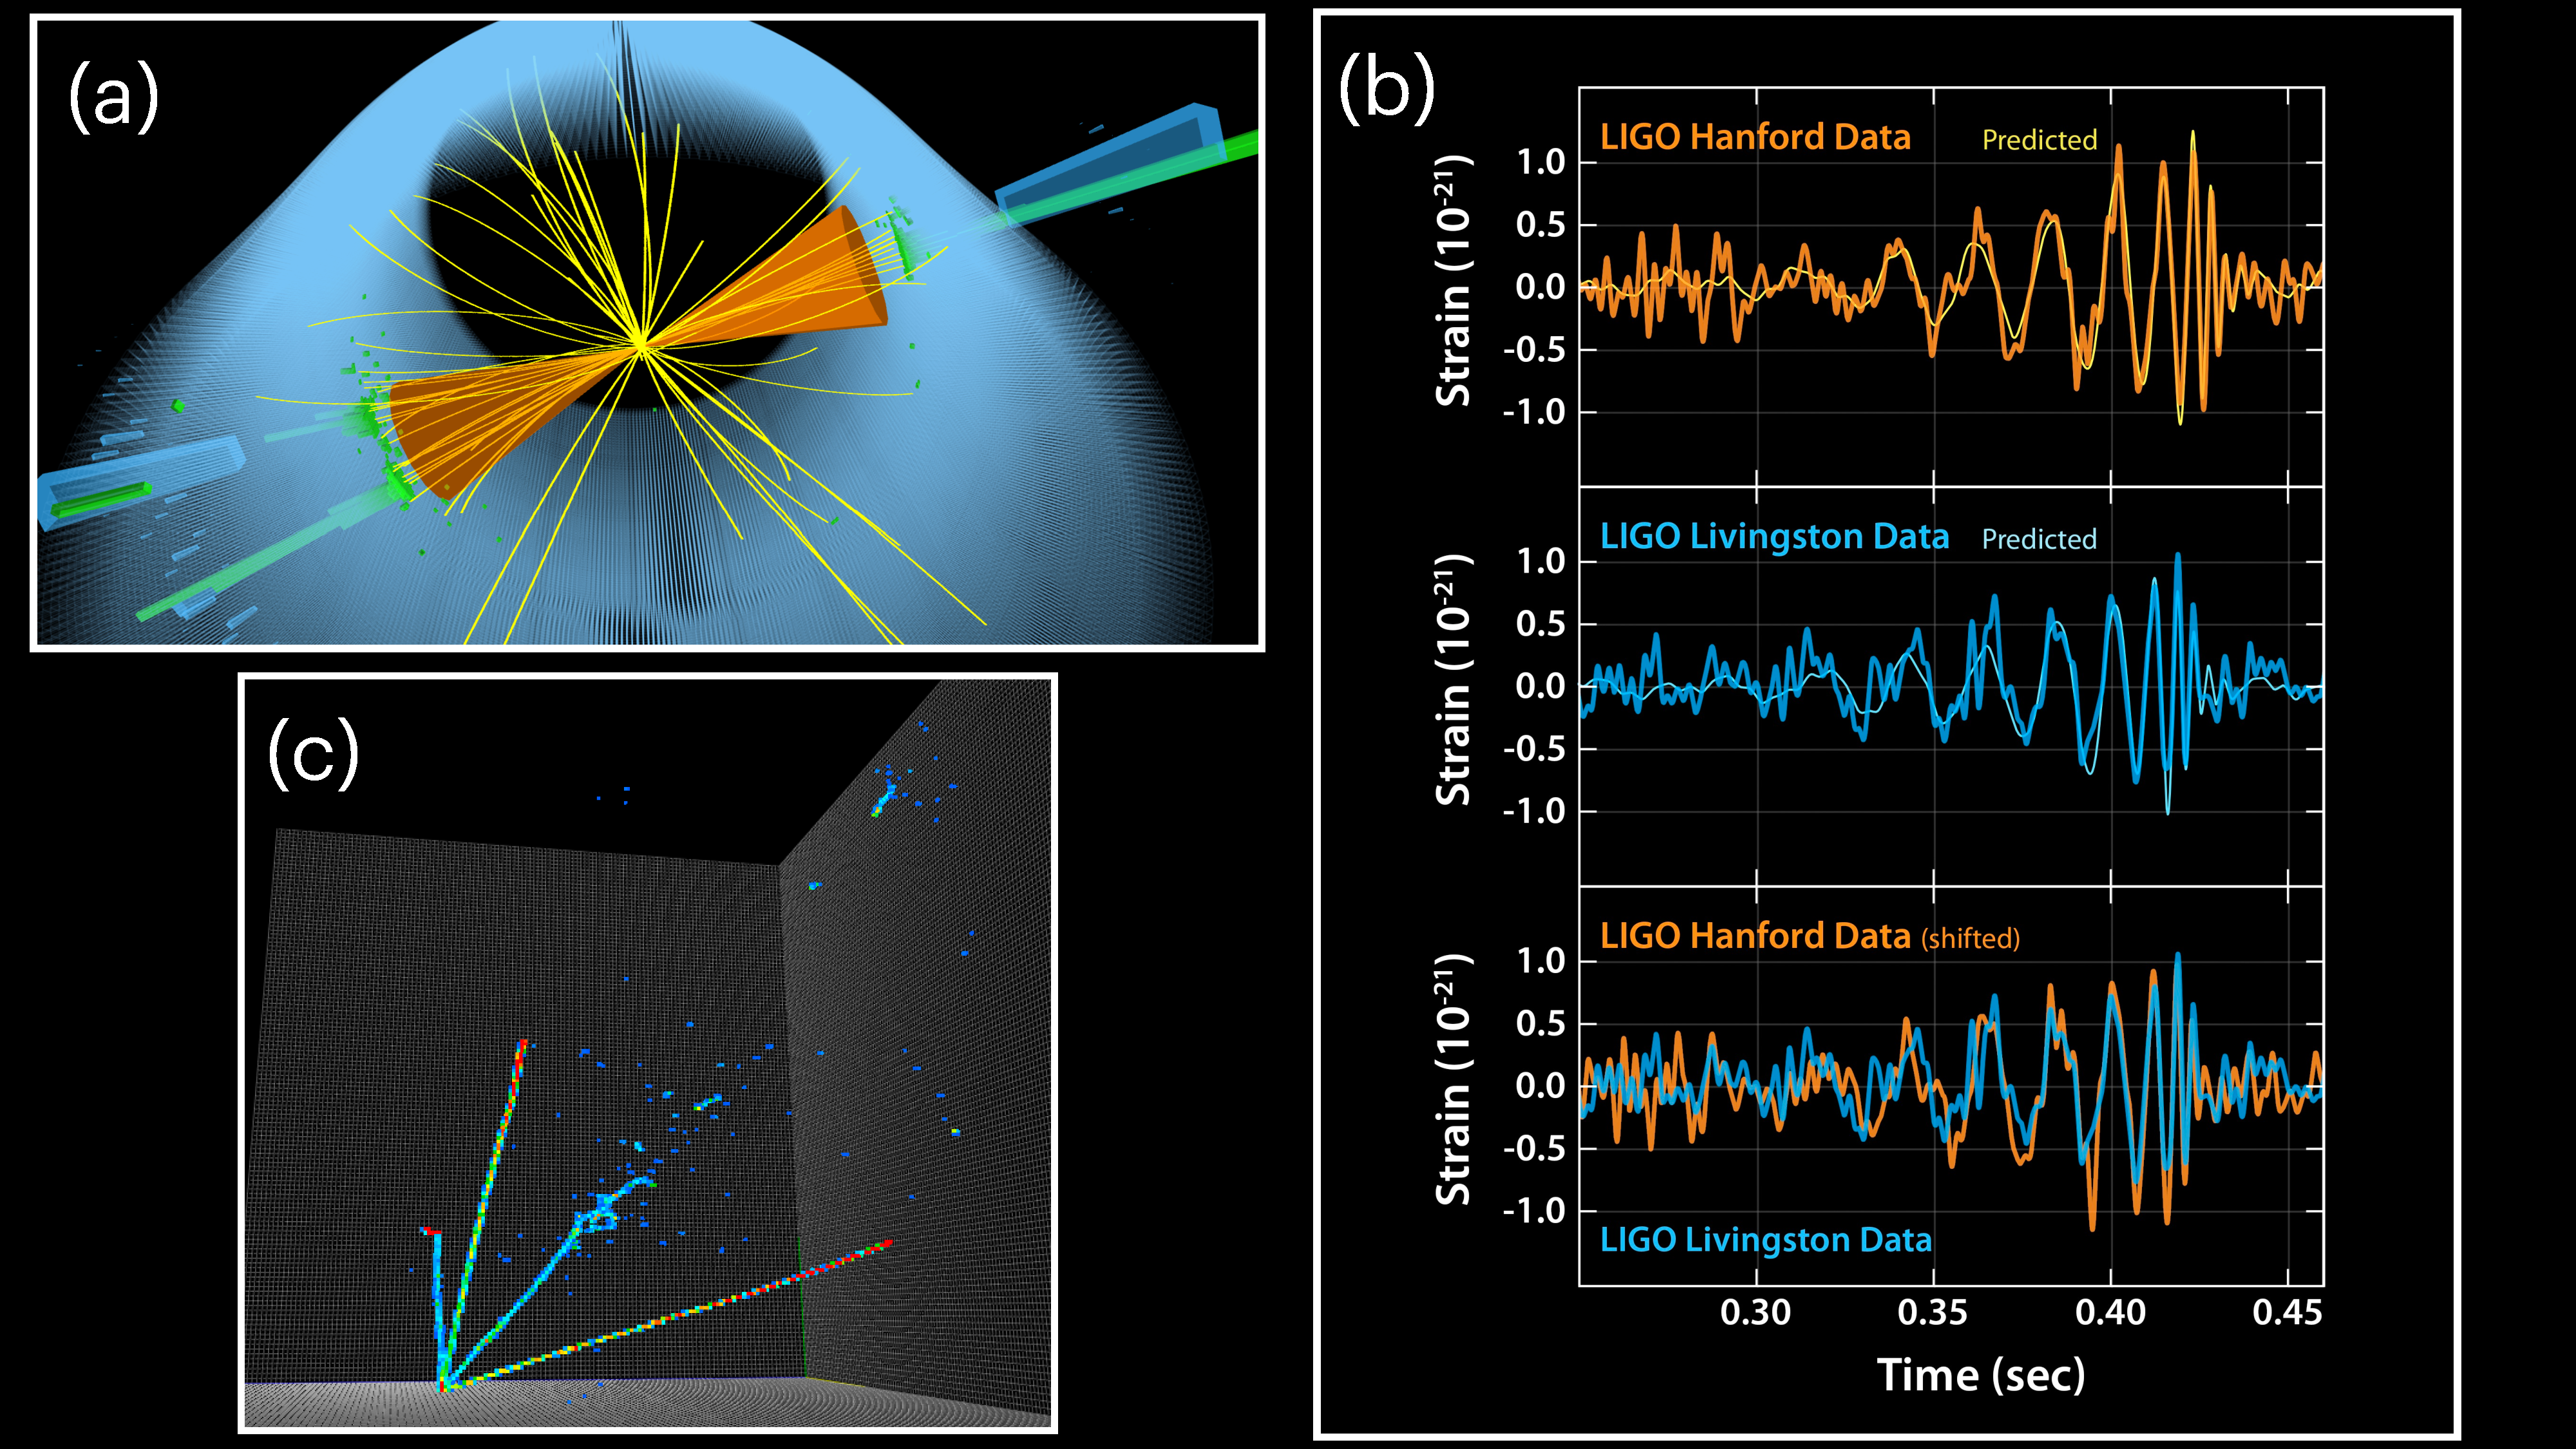
\includegraphics[width=0.5\textwidth]{phys141_data.pdf}
    \caption{Demonstration of the Jupyter Book format used for the ``Particle Physics and Machine Learning'' section of the UCSD Data Science Capstone Course DSC 180AB.
        The code is executable and renders in the browser.
        Visualizations of data sets to be used in Physics 141/241: (a) high-energy collider physics data consisting of simulated particle jets from the CMS experiment for identifying Higgs bosons, (b) astrophysical time-series data consisting of gravitational wave transient events maintained by the LIGO/Virgo/KAGRA collaboration, and (c) neutrino physics data containing simulated neutrinos interacting in a liquid argon time projection chamber (right).
        \label{fig:teaching}}
\end{figure}

Finally, I am also developing a new graduate course with Prof. R. Sekhar Chivukula on computational methods in collider physics, covering beyond the SM physics, Monte Carlo event generators, detector simulation, and ML methods for data analysis.
The goal of the course is to give graduate students an ``end-to-end'' view of the process from theoretical prediction to experimental constraints.

\vspace{-1ex}
\subsection*{Service}

During 2020--2021 and 2021--2022 academic years, I served on the Physics Department Graduate Admissions Committee, and the Equity, Diversity, and Inclusion Committee.
As part of this dual role, I have advocated for the use of holistic review, with a well-defined rubric for evaluating students, including dimensions for EDI contributions.
I was also tasked with additional responsibilities including coordinating the graduate fellowships for URM students.
Beginning in 2022, I also serve as the Physics Department representative to the Equity in Graduate Education (EGE) Consortium, formerly known as the California Consortium for Inclusive Doctoral Education (C-CIDE).

I have served as a peer reviewer for \emph{J. High Energy Phys.}, \emph{Phys. Lett. B}, \emph{Phys. Rev. D}, \emph{Phys. Rev. Research}, \emph{Eur. Phys. J. C}, \emph{Comput. Softw. Big Sci.}, and \emph{Nucl. Instrum. Methods Phys. Res. A}, and \emph{Applied Optics}, and as a Guest Associate Editor for \emph{Front. Big Data} and \emph{Front. AI}.
I have also served as an external reviewer for the Department of Energy and the European Science Foundation.
In 2020 and 2022, I organized the Fast Machine Learning for Science Workshops.
I am actively participating in the Snowmass 2022 process, which defines the priorities for the US HEP program for the next decade.
I coauthored white papers on machine learning for Higgs boson pair production~[\mycite{Apresyan:2022tqw}], GNNs~[\mycite{Thais:2022iok}], fast ML~[\mycite{Harris:2022qtm}], and data science and ML in physics education~[\mycite{Benelli:2022sqn}], as well as the final report from the computational subgroup on AI-specific hardware.

\vspace{-1ex}
\subsection*{Equity, Diversity, and Inclusion}

As a faculty member, I have led Equity, Diversity, and Inclusion (EDI) initiatives, especially promoting equitable graduate admissions.
This involved giving a seminar to the Graduate Admissions Committee on holistic review and other lessons learned from the EGE Consortium.
With other high energy physics faculty members, we developed a common rubric for graduate admissions that we used in the 2021--2022 academic year.
Thanks in part to my efforts at raising awareness of EDI issues, our committee matriculated one of the most diverse graduate classes, with 34\% women and 14\% underrepresented minority (URM) students for the Physics Ph.D. program (excluding the newly created Astronomy Ph.D. program).

As key personnel of the NSF HDR A3D3 Institute, I co-chair the Equity and Career Committee.
One of my main contributions in this role was the conception and execution of the A3D3 Postbaccalaureate Research Fellowship.
This one-year fellowship is intended to increase research opportunities for URM groups in STEM, including African American/Black, Chicanx/Latinx, Native American/Alaska Native, Native Hawaiin/Pacific Islander, and Filipinx scientists.
In particular, the program is intended as a bridge to help students with a lack of access to research opportunities gain experience, while being supported with mentoring and professional development activities (like technical writing seminars), in order to be more competitive for graduate study or industry positions.
In our first year (2022--2023), four postbaccalaureate fellows have been recruited to conduct research at institutions across the country including UCSD, and we hope to grow the program in the coming years.

I have also mentored students ranging from high school to graduate school participating in the SDSC MAP, UCSD EXPAND, UCSD ENLACE, Cal-Bridge, CERN REU, IRIS-HEP fellowship, APS National Mentorship, and US CMS Mentorship programs.
Many of these programs specifically aim to provide opportunities for URM students in STEM.
Finally, I contribute to department-level outreach activities, for example, as an exhibitor for the Physics Department and my lab at the \href{https://www.barriologansae.com/}{Barrio Logan Science \& Art Expo} on Saturday, April 16, 2022.

\vspace{0.1in}
\includegraphics{signature.pdf}\\
\indent\indent Javier M. Duarte

\end{document}
